%%%%%%%%%%%%%%%%%%%%%%%%%%%%%%%%%%%%%%%%%
% Short Sectioned Assignment
% LaTeX Template
% Version 1.0 (5/5/12)
%
% This template has been downloaded from:
% http://www.LaTeXTemplates.com
%
% Original author:
% Frits Wenneker (http://www.howtotex.com)
%
% License:
% CC BY-NC-SA 3.0 (http://creativecommons.org/licenses/by-nc-sa/3.0/)
%
%%%%%%%%%%%%%%%%%%%%%%%%%%%%%%%%%%%%%%%%%

%----------------------------------------------------------------------------------------
%	PACKAGES AND OTHER DOCUMENT CONFIGURATIONS
%----------------------------------------------------------------------------------------

\documentclass[paper=a4, fontsize=12pt]{scrartcl} % A4 paper and 11pt font size

\usepackage[utf8]{inputenc}
%\usepackage{fourier} % Use the Adobe Utopia font for the document - comment this line to return to the LaTeX default
\usepackage[english]{babel} % English language/hyphenation
\usepackage{amsmath,amsfonts,amsthm} % Math packages
\usepackage{graphicx}
\usepackage{sectsty} % Allows customizing section commands
\allsectionsfont{\centering \normalfont\scshape} % Make all sections centered, the default font and small caps

%\usepackage{fancyhdr} % Custom headers and footers
%\pagestyle{fancyplain} % Makes all pages in the document conform to the custom headers and footers
%\fancyhead{} % No page header - if you want one, create it in the same way as the footers below
%\fancyfoot[L]{} % Empty left footer
%\fancyfoot[C]{} % Empty center footer
%\fancyfoot[R]{\thepage} % Page numbering for right footer
%\renewcommand{\headrulewidth}{0pt} % Remove header underlines
%\renewcommand{\footrulewidth}{0pt} % Remove footer underlines
%\setlength{\headheight}{13.6pt} % Customize the height of the header

\numberwithin{equation}{section} % Number equations within sections (i.e. 1.1, 1.2, 2.1, 2.2 instead of 1, 2, 3, 4)
\numberwithin{figure}{section} % Number figures within sections (i.e. 1.1, 1.2, 2.1, 2.2 instead of 1, 2, 3, 4)
\numberwithin{table}{section} % Number tables within sections (i.e. 1.1, 1.2, 2.1, 2.2 instead of 1, 2, 3, 4)

%\setlength\parindent{0pt} % Removes all indentation from paragraphs - comment this line for an assignment with lots of text

%----------------------------------------------------------------------------------------
%	TITLE SECTION
%----------------------------------------------------------------------------------------

\newcommand{\horrule}[1]{\rule{\linewidth}{#1}} % Create horizontal rule command with 1 argument of height

\title{	
\normalfont \normalsize 
\textsc{Hochschule Furtwangen University\\Fakultät Digitale Medien\\Gamedesign Workshop} \\ % Your university, school and/or department name(s)
\horrule{2pt} \\[0.4cm] % Thin top horizontal rule
\huge Fu-Type YAVBWC \\ % The assignment title
\horrule{2pt} \\[0.5cm] % Thick bottom horizontal rule
}

\author{Alexander Scheurer}

\date{\normalsize\today} % Today's date or a custom date

\begin{document}

\maketitle % Print the title

%------------------------------------------------

\section{Introduction}

Fu-Type YAVBWC (Yet another version, but with cards) is a side scrolling 2D action bullet hell shooter with a unique card-power-up mechanic, aimed at casual to hardcore gamers.

%------------------------------------------------

\section{Description}

You start of with a basic ship and nothing else but to play your first level. After finishing the first semi-boss you receive a card which represents a power-up that will automatically be equipped to the first of your three passive power-up slots. After a few more waves of basic enemies, which are now considerably easier then before the difficulty cranks up and you soon find another semi-boss from whom you receive an active power-up. After finishing the final boss for this tutorial level you get five more passive and another active power-up.

All power-ups (more firepower, an additional weapon or different ships) are represented by cards. There are several card tiers, meaning for example a 'rare'  health-up card is stronger as a 'common' one. Also there are different ways to unlock them, like just by completing a stage for a basic card or things like beating a set highscore, doing challenge or even a hidden challenge to unlock higher tiered cards.

To finish the game you'll need nothing more then the basic set, so the casual gamer is not alienated by grinding for cards. But gamers hunting for a highscore will have work to do, getting their cards, as well as putting together an optimal deck (which should differ by level as well as playstyle).

An additional gamemode where you play the game from beginning to end in a rogue-like fashion, just being able to use the cards that drop randomly for you in this run. Players might and should be able to break the game completely when they get good cards, but also the game should be crushingly hard if they get unlucky drops.

%------------------------------------------------

\section{Key features}

Simple but deep mechanic: Everything is as card, but how to mix and match them to get the optimal synergy is not easy.

Different Gamemodes make for a totaly different experience: Just playing the game for the casual gamer, optimizing the deck and going for a new highscore for the hardcore gamer, having a gamble and trying the rogue-like mode for another round.


%------------------------------------------------

\section{Platform(s)}

Since almost all modern platforms can handle a 2D game even with a high visual fidelity there is no limit to on what platform this game can be released.

%------------------------------------------------

\section{Concept art}
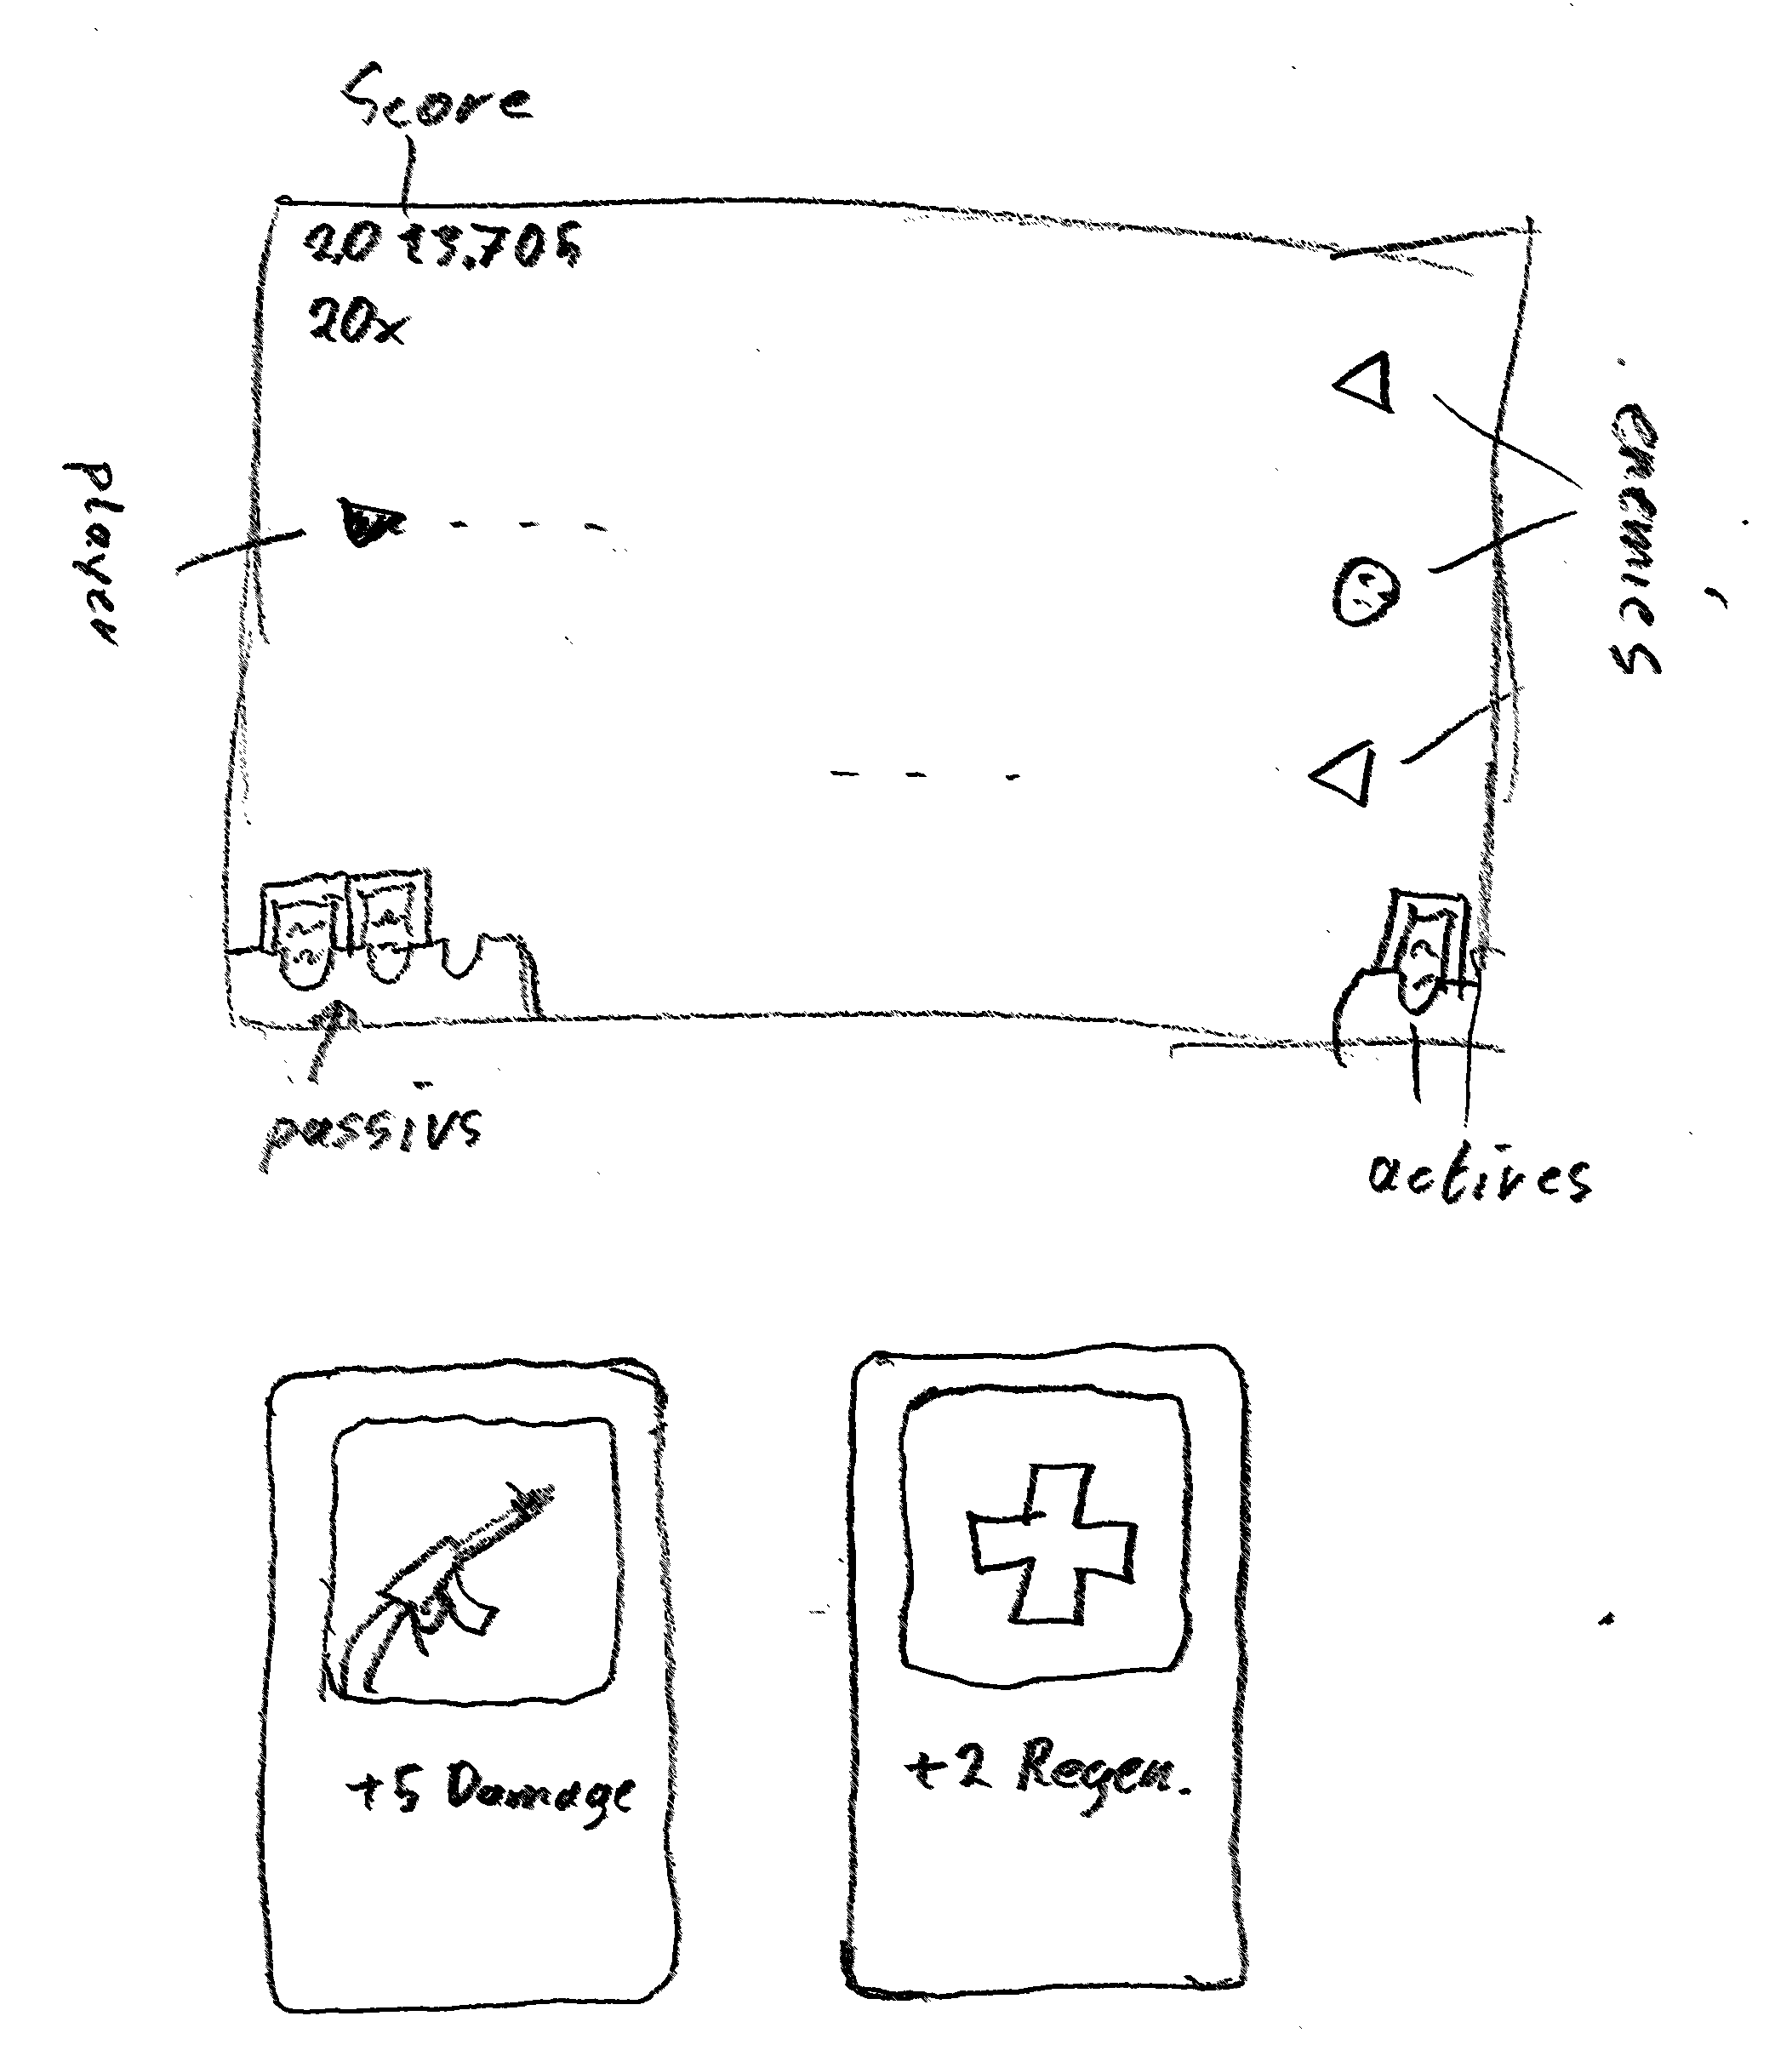
\includegraphics[natwidth=2106,natheight=2416]{conceptart.png}
%------------------------------------------------

\end{document}